% TF_RelFinal.tex
% Trabalho Final - Opção 2: Exemplo 6.2 (Versteeg e Malalasekera) com meio poroso
% Trechos marcados com \pendente{...} ainda precisam ser preenchidos.
\documentclass[11pt,a4paper]{article}

\usepackage[utf8]{inputenc}
\usepackage[T1]{fontenc}
\usepackage[brazil]{babel}
\usepackage[a4paper,margin=2.5cm]{geometry}
\usepackage{amsmath,amssymb}
\usepackage{graphicx}
\usepackage{float}
\usepackage{xcolor}
\usepackage{listings}
\usepackage{hyperref}

\newcommand{\pendente}[1]{\textcolor{red}{\textbf{[PENDENTE: #1]}}}

\lstset{
  language=Python,
  basicstyle=\ttfamily\footnotesize,
  breaklines=true,
  frame=single,
  numbers=left,
  numberstyle=\tiny,
  showstringspaces=false,
  literate={á}{{\'a}}1 {à}{{\`a}}1 {ã}{{\~a}}1 {â}{{\^a}}1 {é}{{\'e}}1 {ê}{{\^e}}1
           {í}{{\'i}}1 {ó}{{\'o}}1 {õ}{{\~o}}1 {ô}{{\^o}}1 {ú}{{\'u}}1 {ç}{{\c c}}1
           {Á}{{\'A}}1 {É}{{\'E}}1 {Í}{{\'I}}1 {Ó}{{\'O}}1 {Ú}{{\'U}}1 {Ç}{{\c C}}1
           {²}{{$^2$}}1 {³}{{$^3$}}1 {–}{{-}}1 {ª}{{\textordfeminine}}1
}

\title{Trabalho Final -- Escoamento em um bocal convergente preenchido com meio poroso: solução pelo algoritmo SIMPLE}
\author{Gustavo Coimbra Vilela}
\date{23/11/2026}

\begin{document}
\maketitle

%======================================================================
\section{Introdução}

Em escoamentos incompressíveis, a pressão não possui uma equação de
transporte própria: ela aparece apenas como termo fonte nas equações da
quantidade de movimento e é determinada, de forma indireta, pela exigência
de que o campo de velocidades conserve a massa. O algoritmo SIMPLE
(\emph{Semi-Implicit Method for Pressure-Linked Equations}), proposto por
Patankar e Spalding, resolve esse acoplamento de forma iterativa: a
equação da quantidade de movimento fornece a velocidade a partir de uma
pressão estimada, e a equação da continuidade é transformada em uma equação
de correção para a pressão.

Escoamentos através de meios porosos ocorrem em filtros, reatores de leito
fixo, trocadores regenerativos e sistemas de armazenamento de energia
térmica em leitos de cápsulas. Nesses casos, a interação do fluido com a
matriz sólida produz uma força de arrasto distribuída, descrita pelas leis
de Darcy e de Forchheimer, que se soma às forças presentes no escoamento
livre.

O objetivo deste trabalho é implementar o algoritmo SIMPLE, em malha
deslocada e com $N$ volumes genérico, para o escoamento unidimensional em um
bocal convergente (Exemplo 6.2 de Versteeg e Malalasekera
\cite{versteeg}); avaliar o comportamento do método quanto ao refino de
malha, ao fator de sub-relaxação e ao critério de convergência; e, em
seguida, estender o modelo para o caso em que o bocal está preenchido com um
leito de esferas compactadas.

%======================================================================
\section{O Problema Físico e o Modelo Matemático}

\subsection{Problema físico}

O escoamento ocorre em um bocal plano convergente de comprimento
$L=2{,}0$~m, cuja área da seção transversal varia linearmente de
$A_A=0{,}5$~m$^2$ na entrada a $A_E=0{,}1$~m$^2$ na saída:
\begin{equation}
  A(x)=0{,}5-0{,}2\,x \quad [\mathrm{m^2}] .
\end{equation}
Na entrada, o fluido provém de um reservatório em repouso com pressão de
estagnação $p_0=10$~Pa; na saída, ele é descarregado como jato livre, com
pressão estática $p_E=0$~Pa. A massa específica é $\rho=1$~kg/m$^3$.

Na segunda parte do trabalho, o bocal é preenchido com um leito de esferas
compactadas de porosidade $\varepsilon=0{,}36$ e diâmetro $D_p$
\pendente{valor de $D_p$}, e o fluido passa a ter viscosidade $\mu$
\pendente{fluido e valor de $\mu$}.

\subsection{Hipóteses simplificativas}

\begin{enumerate}
  \item Regime permanente.
  \item Escoamento incompressível ($\rho$ constante).
  \item Escoamento unidimensional: propriedades uniformes em cada seção
        transversal, variando apenas com $x$.
  \item Sem atrito nas paredes do bocal (o fluido é tratado como invíscido
        no escoamento livre).
  \item No caso poroso: meio homogêneo, isotrópico e rígido, com o leito
        ocupando todo o bocal a partir de $x=0$; a interação fluido-sólido é
        representada pelo arrasto de Darcy-Forchheimer, e a velocidade $u$
        é a velocidade de Darcy (superficial), $u=Q/A$.
  \item No caso poroso, o termo convectivo é escrito com a velocidade de
        Darcy, sem o fator $1/\varepsilon^2$ da formulação por média
        volumétrica \pendente{justificar por ordem de grandeza com os
        valores de $D_p$ e $\mu$ adotados}.
\end{enumerate}

\subsection{Equações governantes}

Com as hipóteses acima, as equações da continuidade e da quantidade de
movimento reduzem-se a
\begin{equation}
  \frac{d}{dx}\left(\rho\,u\,A\right)=0 ,
  \label{eq:cont}
\end{equation}
\begin{equation}
  \rho\,u\,A\,\frac{du}{dx}
  =-A\,\frac{dp}{dx}
  -A\left(\frac{\mu}{K}\,u+\frac{C_E\,\rho}{\sqrt{K}}\,|u|\,u\right) .
  \label{eq:mom}
\end{equation}
O último termo é a força de arrasto exercida pela matriz porosa por
unidade de volume. Para o bocal sem meio poroso, $K\to\infty$ e esse termo
se anula. Com área constante, a Eq.~\eqref{eq:cont} impõe $du/dx=0$ e a
Eq.~\eqref{eq:mom} recai na lei de Darcy-Forchheimer,
\begin{equation}
  -\frac{\Delta p}{L}=\frac{\mu}{K}\,U+\frac{C_E}{\sqrt{K}}\,\rho\,U^2 .
\end{equation}

A permeabilidade $K$ (m$^2$) e a constante de Ergun $C_E$ do leito de
esferas são dadas pela correlação de Ergun:
\begin{equation}
  K=\frac{\varepsilon^3\,D_p^2}{150\,(1-\varepsilon)^2},
  \qquad
  C_E=\frac{1{,}75}{\sqrt{150\,\varepsilon^3}} .
  \label{eq:ergun}
\end{equation}
O termo linear (Darcy) representa o atrito viscoso nas superfícies das
esferas e pode ser obtido modelando o leito como um feixe de capilares
com o diâmetro hidráulico
$D_H=\tfrac{2}{3}\,\varepsilon D_p/(1-\varepsilon)$ (modelo de
Kozeny-Carman); o termo quadrático (Forchheimer) representa as perdas
inerciais nas sucessivas expansões e contrações dos poros.
\pendente{valores de $K$, $C_E$ e $\mathrm{Re}_d=\rho U D_p/\mu$}

\subsection{Condições de contorno}

\begin{itemize}
  \item \textbf{Entrada ($x=0$):} pressão de estagnação $p_0$. Entre o
        reservatório e a entrada, a equação de Bernoulli fornece
        \begin{equation}
          p_A=p_0-\tfrac12\,\rho\,u_A^2 .
          \label{eq:bern}
        \end{equation}
        A pressão estática na entrada não é conhecida a priori, pois depende
        da velocidade calculada.
  \item \textbf{Saída ($x=L$):} pressão estática $p_E=0$.
\end{itemize}

\subsection{Solução analítica}

Sem meio poroso, a pressão de estagnação se conserva ao longo do bocal, e
com $p_E=0$:
\begin{equation}
  \dot m=\rho\,A_E\sqrt{\frac{2\,p_0}{\rho}}=0{,}44721~\mathrm{kg/s},
  \qquad
  u(x)=\frac{\dot m}{\rho\,A(x)},
  \qquad
  p(x)=p_0-\tfrac12\,\rho\,u(x)^2 .
  \label{eq:exata}
\end{equation}

Com meio poroso, como $\dot m$ é constante e $A(x)$ é linear, a
Eq.~\eqref{eq:mom} pode ser integrada analiticamente de $x=0$ a $x=L$.
\pendente{dedução e expressão da equação do 2º grau em $\dot m$}

%======================================================================
\section{Implementação Numérica}

\subsection{Malha}

Adotou-se uma malha deslocada (\emph{staggered}). O domínio é dividido em
$N$ volumes de pressão de largura $\Delta x=L/N$, com $N+1$ nós de pressão
nas posições $x_I=(I-1)\,\Delta x$, $I=1,\dots,N+1$ (nós $A$ a $E$ no caso
$N=4$ do livro). Os $N$ pontos de velocidade ficam nas faces dos volumes de
pressão, em $x_i=(i-\tfrac12)\,\Delta x$, $i=1,\dots,N$. Assim:
\begin{itemize}
  \item o volume de controle da \textbf{continuidade} é centrado em um nó
        de pressão, e suas faces coincidem com pontos de velocidade;
  \item o volume de controle da \textbf{quantidade de movimento} é centrado
        em um ponto de velocidade, e suas faces coincidem com nós de pressão.
\end{itemize}
Com esse arranjo, cada equação dispõe, nas suas faces, exatamente da
variável armazenada pela outra malha: a diferença de pressão que acelera o
fluido e a vazão que atravessa as faces são obtidas sem interpolação, o que
evita o desacoplamento entre pressão e velocidade (campo ``tabuleiro de
xadrez'').

Nas equações a seguir usa-se a notação local: $P$ é o ponto central do
volume, $W$ e $E$ seus vizinhos, e $w$ e $e$ suas faces.

\subsection{Formulação temporal}

O problema é permanente e não há termo temporal. As iterações do SIMPLE
funcionam como um processo de pseudotempo até que as equações discretizadas
sejam satisfeitas.

\subsection{Funções de interpolação}

\begin{itemize}
  \item \textbf{Termo advectivo:} esquema \emph{upwind} (UDS) para a
        velocidade transportada. Como $u>0$ em todo o bocal,
        $u_w=u_W$ e $u_e=u_P$.
  \item \textbf{Vazões nas faces:} interpolação linear entre os pontos de
        velocidade vizinhos,
        $F_w=\rho\,A_w\,(u_W+u_P)/2$ e $F_e=\rho\,A_e\,(u_P+u_E)/2$,
        calculadas com as velocidades da iteração anterior.
  \item \textbf{Termo difusivo:} não há, pois o escoamento é tratado como
        invíscido nas paredes.
  \item \textbf{Termo de arrasto (fonte):} regra do ponto médio, com o
        integrando avaliado no centro do volume.
\end{itemize}

\subsection{Discretização da quantidade de movimento}

Integrando a Eq.~\eqref{eq:mom} de $w$ a $e$:
\begin{equation}
  F_e\,u_P-F_w\,u_W=(p_w-p_e)\,A_P-D_P\,u_P ,
  \qquad
  D_P=\left(\frac{\mu}{K}+\frac{C_E\,\rho\,|u_P^{old}|}{\sqrt{K}}\right)A_P\,\Delta x .
\end{equation}
O termo $|u_P|$ do arrasto de Forchheimer é avaliado com a velocidade da
iteração anterior. Como o arrasto é proporcional a $-u_P$ com $D_P>0$, ele é
incorporado ao coeficiente central, o que reforça a dominância diagonal.
Resulta a forma geral
\begin{equation}
  \boxed{\;a_P\,u_P=a_W\,u_W+a_E\,u_E+S_u\;}
\end{equation}

\paragraph{Pontos internos ($2\le i\le N-1$).}
\[
  a_W=F_w,\qquad a_E=0,\qquad
  a_P=a_W+a_E+(F_e-F_w)+D_P=F_e+D_P,\qquad
  S_u=(p_w-p_e)\,A_P .
\]

\paragraph{Ponto 1 (entrada).}
A face oeste coincide com o nó $A$, onde a pressão é dada pela
Eq.~\eqref{eq:bern} e, pela continuidade, $u_A=u_1\,A_1/A_A$. Substituindo
na equação do ponto 1 e linearizando $u_A^2$ com $F_A=\rho\,u_A A_A$ da
iteração anterior, a contribuição negativa ao coeficiente central foi
transferida para o termo fonte com $u_1^{old}$ (correção adiada), para
manter $a_P>0$ mesmo com estimativas iniciais ruins:
\[
  a_W=0,\qquad a_E=0,\qquad
  a_P=F_e+F_A\,\tfrac12\left(\frac{A_1}{A_A}\right)^2+D_P,\qquad
  S_u=(p_0-p_e)\,A_1+F_A\,\frac{A_1}{A_A}\,u_1^{old} .
\]

\paragraph{Ponto $N$ (saída).}
A face leste coincide com o nó de saída, onde não há ponto de velocidade
vizinho; a vazão é obtida pela continuidade, $F_e=\rho\,u_N A_N$:
\[
  a_W=F_w,\qquad a_E=0,\qquad a_P=F_e+D_P,\qquad
  S_u=(p_w-p_E)\,A_N .
\]

O coeficiente usado na correção de velocidade é $d_P=A_P/a_P$, calculado
após a inclusão de $D_P$.

\subsection{Equação de correção da pressão}

Escrevendo $p=p^*+p'$ e $u=u^*+u'$ e subtraindo a equação da quantidade
de movimento com $p^*$ da equação com $p$, obtém-se, desprezando as
correções dos vizinhos (aproximação do SIMPLE),
\begin{equation}
  u_P=u_P^*+d_P\,(p'_w-p'_e) .
\end{equation}
Substituindo essa expressão na continuidade discretizada,
$(\rho uA)_e-(\rho uA)_w=0$, em cada volume de pressão:
\begin{equation}
  a_P\,p'_P=a_W\,p'_W+a_E\,p'_E+b',
  \qquad
  a_W=(\rho\,d\,A)_w,\quad a_E=(\rho\,d\,A)_e,\quad
  a_P=a_W+a_E,\quad b'=F_w^*-F_e^* ,
\end{equation}
em que $b'$ é o desbalanço de massa do volume calculado com $u^*$.
Nos nós de contorno adota-se $p'_A=p'_E=0$: em $E$ a pressão é prescrita,
e em $A$ ela é determinada por $p_0$ e $u_1$ pela Eq.~\eqref{eq:bern},
sendo recalculada a cada iteração.

\subsection{Algoritmo}

\begin{enumerate}
  \item Estimar $p^*$ (linear entre 10 e 0~Pa) e $u$ (a partir de
        $\dot m=1$~kg/s).
  \item Calcular $F$, $D_P$, os coeficientes $a_P$, $a_W$, $S_u$ e $d_P$.
  \item Calcular o resíduo da quantidade de movimento e verificar a
        convergência.
  \item Resolver a quantidade de movimento pelo TDMA, obtendo $u^*$.
  \item Calcular $b'$ e resolver a correção de pressão pelo TDMA,
        obtendo $p'$.
  \item Corrigir: $p=p^*+p'$ e $u=u^*+d\,(p'_w-p'_e)$.
  \item Sub-relaxar: $u^{new}=(1-\alpha)\,u^{old}+\alpha\,u$ e
        $p^{new}=(1-\alpha)\,p^{old}+\alpha\,p$, com o mesmo fator $\alpha$.
  \item Recalcular $p_A$ pela Eq.~\eqref{eq:bern} com a velocidade
        sub-relaxada.
  \item Tomar $u^{new}$ e $p^{new}$ como nova estimativa e voltar ao
        passo~2.
\end{enumerate}
A iteração também é interrompida se alguma velocidade divergir (valor não
finito ou superior a $10^6$~m/s) ou se for atingido o número máximo de
iterações (20\,000), casos em que a simulação é registrada como não
convergida.

\subsection{Cálculo do resíduo}

No início de cada iteração, os coeficientes montados com os campos da
iteração anterior são aplicados a esses mesmos campos, e o resíduo de cada
ponto de velocidade é o desbalanço da equação discretizada:
\begin{equation}
  R=\sum_{i=1}^{N}\left|\,a_{P,i}\,u_i-a_{W,i}\,u_{i-1}-S_{u,i}\,\right| ,
\end{equation}
com $a_{W,1}=0$. Usa-se a soma dos valores absolutos para evitar que
resíduos de sinais opostos se cancelem. A solução é aceita quando
$R<\varepsilon_R$, com $\varepsilon_R=10^{-5}$ salvo indicação em
contrário.

%======================================================================
\section{Resultados e Discussões}

Os tempos de processamento apresentados foram medidos apenas no laço
iterativo, com \texttt{time.perf\_counter()} \pendente{processador da
máquina usada}.

\subsection{Verificação com o exemplo do livro}

Com $N=4$ e $\alpha=0{,}8$, o código reproduz a solução convergida
apresentada por Versteeg e Malalasekera (Tabela~\ref{tab:livro}).

\begin{table}[H]
\centering
\caption{Solução convergida para $N=4$: presente trabalho, livro
\cite{versteeg} e solução exata, Eq.~\eqref{eq:exata}.}
\label{tab:livro}
\begin{tabular}{lrrrr}
\hline
Nó de pressão & $A$ & $B$ & $C$ & $D$\\
\hline
$p$ (Pa), presente   & 9,22571 & 9,00418 & 8,25060 & 6,19427\\
$p$ (Pa), livro      & 9,22569 & 9,00415 & 8,25054 & 6,19423\\
$p$ (Pa), exata      & 9,60000 & 9,37500 & 8,88889 & 7,50000\\
\hline
Ponto de velocidade & 1 & 2 & 3 & 4\\
\hline
$u$ (m/s), presente  & 1,38269 & 1,77774 & 2,48883 & 4,14806\\
$u$ (m/s), livro     & 1,38265 & 1,77775 & 2,48885 & 4,14808\\
$u$ (m/s), exata     & 0,99381 & 1,27775 & 1,78885 & 2,98142\\
\hline
\end{tabular}
\end{table}

As diferenças em relação ao livro estão na quinta casa decimal, compatíveis
com o critério de parada. O erro de 39,1\% em relação à solução exata é
igual em todos os pontos de velocidade: satisfeita a continuidade, tem-se
$u_i=\dot m/(\rho A_i)$, de modo que a forma do perfil é exata e todo o erro
está na vazão, $\dot m=0{,}62221$~kg/s. Observou-se, contudo, que os
coeficientes da segunda iteração apresentados no livro para o ponto~1
($a_P=1{,}20425$; $S_u=1{,}98592$) não são reproduzidos (obteve-se
$1{,}14360$ e $1{,}83042$), embora a primeira iteração e a solução
convergida coincidam; a mesma discrepância é relatada por outros usuários
\cite{cfdonline}.

\subsection{Estudo da sub-relaxação}

A Tabela~\ref{tab:relax} e a Figura~\ref{fig:relax} mostram o número de
iterações necessário para a convergência em função de $\alpha$, para
diferentes malhas.

\begin{table}[H]
\centering
\caption{Iterações até a convergência ($\varepsilon_R=10^{-5}$). X: não
convergiu (divergência ou oscilação sem queda do resíduo). Em negrito, o
menor número de iterações de cada malha.}
\label{tab:relax}
\begin{tabular}{c|rrrrrrr}
\hline
$N$ $\backslash$ $\alpha$ & 0,8 & 0,5 & 0,2 & 0,1 & 0,05 & 0,02 & 0,01\\
\hline
2  & \textbf{10} & 21  & 58  & 114 & 235 & 599 & 1206\\
4  & \textbf{28} & 30  & 81  & 166 & 337 & 849 & 1703\\
8  & X  & 185 & \textbf{103} & 210 & 424 & 1066 & 2136\\
16 & X  & X   & 661 & \textbf{230} & 459 & 1145 & 2290\\
32 & X  & X   & X   & X   & \textbf{487} & 1208 & 2409\\
64 & X  & X   & X   & X   & X   & \textbf{1262} & 2507\\
\hline
\end{tabular}
\end{table}

\begin{figure}[H]
\centering
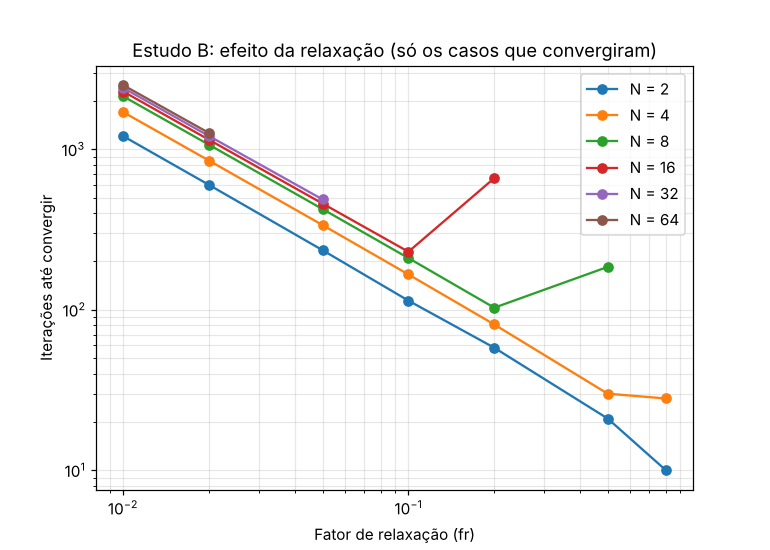
\includegraphics[width=0.7\textwidth]{fig_relaxacao.png}
\caption{Iterações até a convergência em função do fator de sub-relaxação.
Os pontos ausentes correspondem a casos que não convergiram.}
\label{fig:relax}
\end{figure}

Três comportamentos se destacam:
\begin{itemize}
  \item \textbf{O maior $\alpha$ admissível diminui com o refino}, de 0,8
        para $N=4$ a cerca de 0,02 para $N=64$, aproximadamente pela
        metade a cada vez que $N$ dobra. A causa está na aproximação do
        SIMPLE: ao desprezar $\sum a_{nb}u'_{nb}$, supõe-se que a
        velocidade responda apenas à diferença de pressão local. Neste
        problema, porém, $a_W=F_w\approx a_P=F_e$, e o termo desprezado é
        da mesma ordem do termo mantido: a correção de velocidade se acumula
        ao longo da cadeia de pontos a montante. A resposta real da
        velocidade à pressão é, assim, da ordem de $N$ vezes maior que a
        suposta pelo SIMPLE, que superestima $p'$; para não ultrapassar a
        solução, é preciso aplicar uma fração $\alpha\sim1/N$ da correção.
  \item \textbf{O $\alpha$ mais rápido não é o maior que converge.} Próximo
        ao limite de estabilidade a solução oscila antes de convergir
        (por exemplo, $N=16$: 661 iterações com $\alpha=0{,}2$ e 230 com
        $\alpha=0{,}1$), o que dá às curvas da Figura~\ref{fig:relax} o
        formato em ``V''.
  \item \textbf{Abaixo do ótimo, as iterações crescem com $1/\alpha$}
        (inclinação $-1$ na Figura~\ref{fig:relax}): um valor de $\alpha$
        pequeno ``por segurança'' tem custo proporcional.
\end{itemize}

\subsection{Estudo de malha}

Para cada malha, utilizou-se o fator de sub-relaxação que minimizou o
número de iterações (Tabela~\ref{tab:malha}).

\begin{table}[H]
\centering
\caption{Estudo de malha, problema sem meio poroso ($\varepsilon_R=10^{-5}$).}
\label{tab:malha}
\begin{tabular}{rrrrrr}
\hline
$N$ & $\alpha$ & Iterações & Tempo (s) & $\dot m$ (kg/s) & Erro (\%)\\
\hline
4   & 0,8   & 28   & 0,0003 & 0,62221 & 39,13\\
8   & 0,3   & 79   & 0,0012 & 0,53032 & 18,58\\
16  & 0,15  & 224  & 0,0046 & 0,48707 & 8,91\\
32  & 0,05  & 487  & 0,0196 & 0,46659 & 4,33\\
64  & 0,03  & 894  & 0,0702 & 0,45674 & 2,13\\
128 & 0,015 & 1824 & 0,2723 & 0,45194 & 1,06\\
256 & 0,007 & 3887 & 1,2122 & 0,44956 & 0,53\\
\hline
\end{tabular}
\end{table}

\begin{figure}[H]
\centering
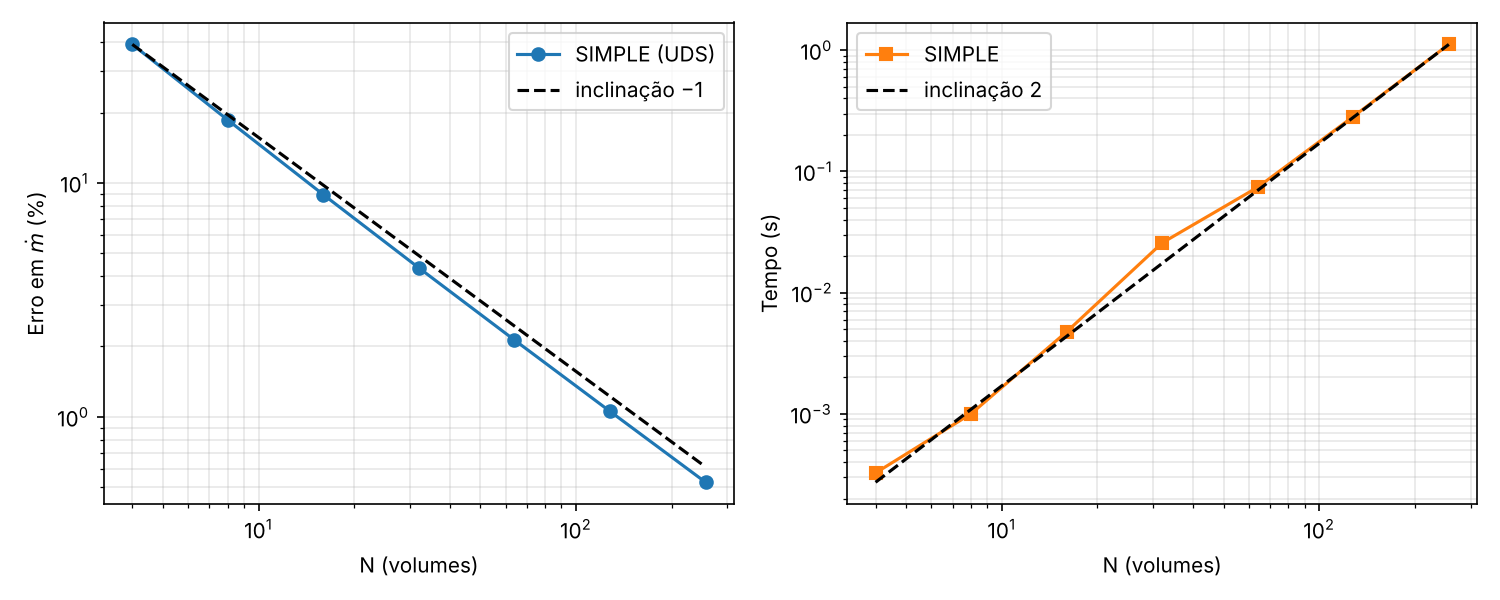
\includegraphics[width=0.95\textwidth]{fig_malha.png}
\caption{Erro na vazão (esquerda) e tempo de processamento (direita) em
função do número de volumes.}
\label{fig:malha}
\end{figure}

O erro cai pela metade a cada vez que a malha é dobrada (inclinação $-1$
na Figura~\ref{fig:malha}), o comportamento esperado de um esquema de
primeira ordem como o UDS. O tempo de processamento cresce com $N^2$: o
custo de cada iteração é proporcional a $N$ (o TDMA é linear em $N$), e o
número de iterações também cresce com $N$, consequência direta da redução
de $\alpha$ discutida acima. Assim, reduzir o erro pela metade custa
quatro vezes mais tempo.

\begin{figure}[H]
\centering
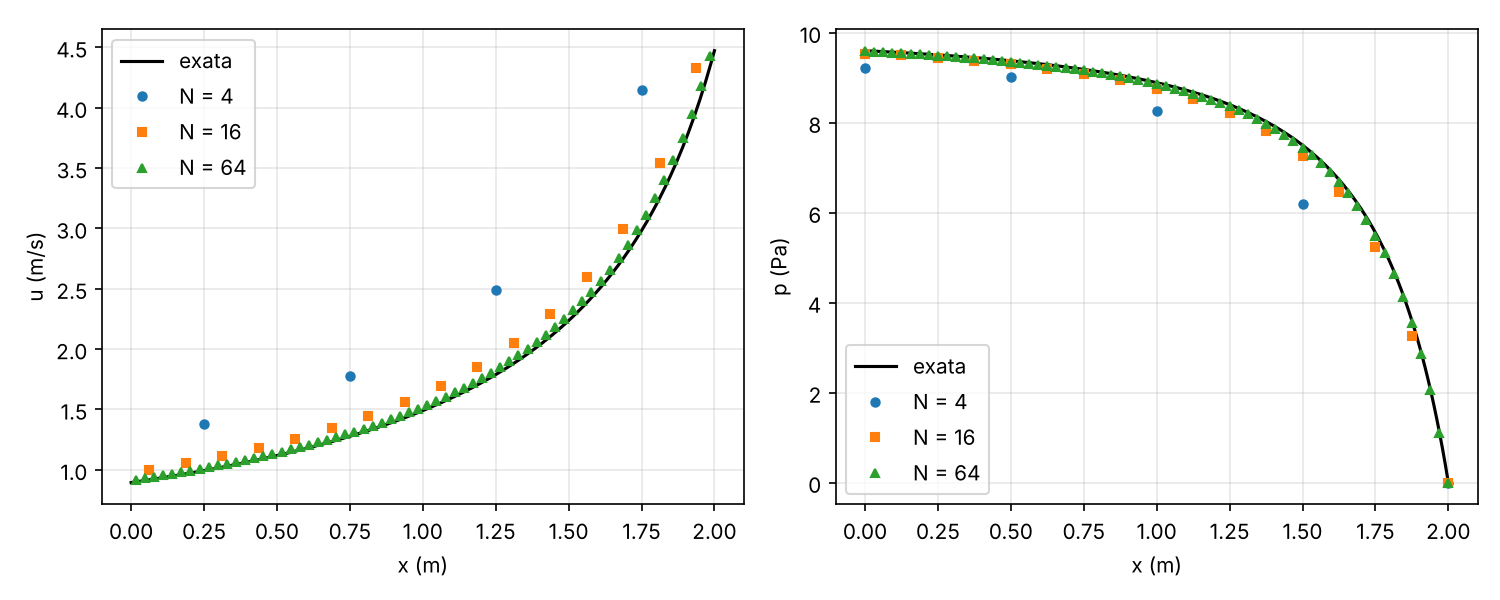
\includegraphics[width=0.95\textwidth]{fig_perfis.png}
\caption{Perfis de velocidade (esquerda) e de pressão (direita) para
diferentes malhas, comparados com a solução exata.}
\label{fig:perfis}
\end{figure}

A Figura~\ref{fig:perfis} mostra que as malhas grosseiras superestimam a
velocidade e subestimam a pressão ao longo de todo o bocal. A causa está no
UDS: o momento que deixa cada volume é transportado com a velocidade do
ponto a montante, inferior à velocidade real na face, em um escoamento que
acelera continuamente. O fluxo de momento na saída é, portanto,
subestimado, e a mesma diferença de pressão produz uma vazão maior que a
real.

\subsection{Estudo do critério de convergência}

\pendente{tabela com $\varepsilon_R=10^{-3}$ a $10^{-7}$ para um $N$ fixo:
iterações, tempo e $\dot m$; discutir a partir de que valor o erro de
iteração fica desprezível frente ao erro de discretização}

\subsection{Bocal preenchido com meio poroso}

\pendente{validação para área constante (Forchheimer) e com a solução
analítica do bocal; estudo de malha e de sub-relaxação com o meio poroso;
perfis de $u$ e $p$ com e sem meio poroso; efeito de $D_p$}

%======================================================================
\section{Considerações Finais}

\begin{itemize}
  \item O algoritmo SIMPLE em malha deslocada, com $N$ volumes genérico,
        reproduziu a solução convergida do Exemplo 6.2 de Versteeg e
        Malalasekera.
  \item O erro na vazão é de primeira ordem em $\Delta x$, como esperado
        para o esquema \emph{upwind}, e cai de 39\% com 4 volumes para
        0,5\% com 256 volumes.
  \item O fator de sub-relaxação admissível diminui aproximadamente com
        $1/N$, devido à aproximação do SIMPLE que despreza as correções dos
        vizinhos. Como consequência, o tempo de processamento cresce com
        $N^2$, e o melhor desempenho é obtido com $\alpha$ um pouco abaixo
        do limite de estabilidade.
  \item \pendente{conclusões do critério de convergência e do meio poroso}
\end{itemize}

%======================================================================
\begin{thebibliography}{9}

\bibitem{versteeg}
H.~K. Versteeg e W.~Malalasekera.
\emph{An Introduction to Computational Fluid Dynamics: The Finite Volume
Method}. 2.\,ed. Harlow: Pearson, 2007.

\bibitem{patankar}
S.~V. Patankar.
\emph{Numerical Heat Transfer and Fluid Flow}.
New York: Hemisphere, 1980.

\bibitem{ergun}
S.~Ergun.
Fluid flow through packed columns.
\emph{Chemical Engineering Progress}, v.~48, p.~89--94, 1952.

\bibitem{darcy}
H.~Darcy.
\emph{Les Fontaines Publiques de la Ville de Dijon}.
Paris: Victor Dalmont, 1856.

\bibitem{forchheimer}
P.~Forchheimer.
Wasserbewegung durch Boden.
\emph{Zeitschrift des Vereines Deutscher Ingenieure}, v.~45,
p.~1782--1788, 1901.

\bibitem{cfdonline}
CFD Online.
Finite Volume -- SIMPLE Algorithm (fórum).
Disponível em: \url{https://www.cfd-online.com/Forums/main/16136-finite-volume-simple-algorithm.html}.

\end{thebibliography}

%======================================================================
\appendix
\section{Código desenvolvido}

\lstinputlisting{simple_bocal.py}

\end{document}
